\chapter{Brugermanual} \label{chap:Brugermanual}

Dette afsnit fungere som en vejledning til opsætning og anvendelse af spillet. Projektet er opbygget som et sammenspil mellem software og hardware, hvor begge dele afhænger af hinanden for at fungere som ønsket.
Inden spillet kan spilles, skal de nødvendige software indstillinger konfigureres. Herunder valg af input, kalibrering samt de korrekte forbindelser mellem applikationen og de fysiske komponenter. Disse indstillinger er med til at sikre, at spillet kan modtage og fortolke dataet fra hardwaren på en sikker og ensartet måde. 
For at opnå dette kræves der en række forberedende trin, som gennemgås i de følgende underafsnit.

\section{Hardware konfiguration} \label{chap:Brugermanual_sec:hardwear}
\vspace{0.5em}

For at køre spillet skal følgende hardware-komponenter andvendes:

\begin{itemize}
    \setlength{\itemsep}{4pt}
    \setlength{\parskip}{0pt}
    \setlength{\parsep}{0pt}
    \item NUCLEO-F302R8 mikrokontroller
    \item MBED Extension board (monteret direkte på Nucleo-boardet)
    \item 30010 Joystick (med tilhørende knapper)
    \item USB kabel
    \item Computer med USB port
\end{itemize}

\begin{figure}[h]
    \centering
    \begin{minipage}{0.33\textwidth}
        \centering
        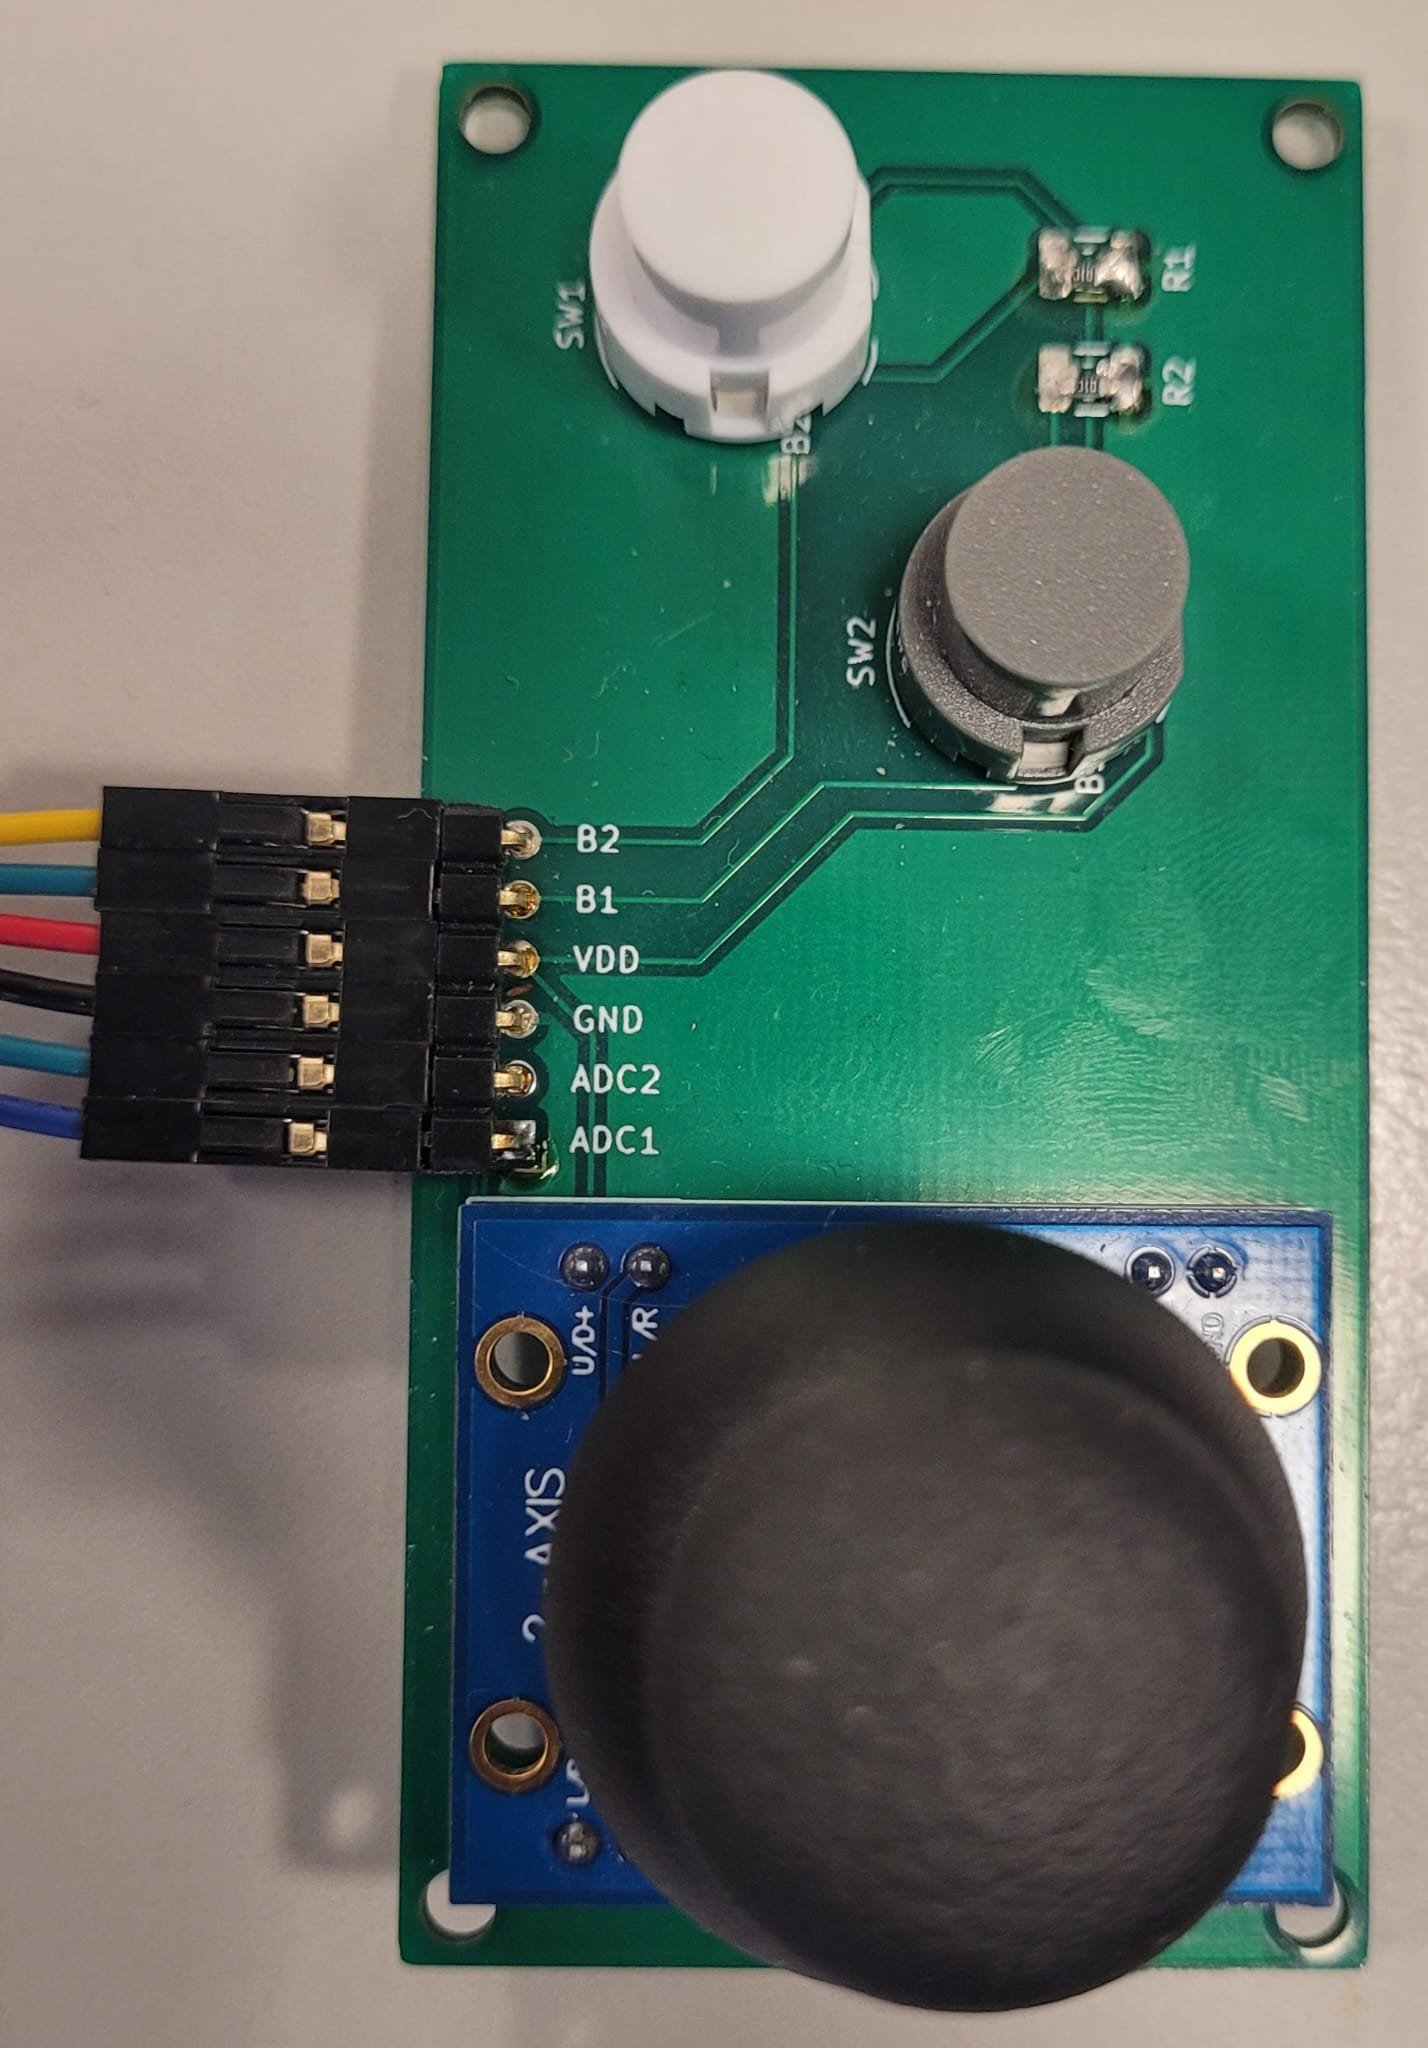
\includegraphics[width=\textwidth]{Picturs/Opsetning/30010joy.jpeg}
        \caption{Billede af 30010-Joystick}
        \label{fig:30010}
    \end{minipage}
    \hspace{0.02\textwidth}
    \begin{minipage}{0.40\textwidth}
        \centering
        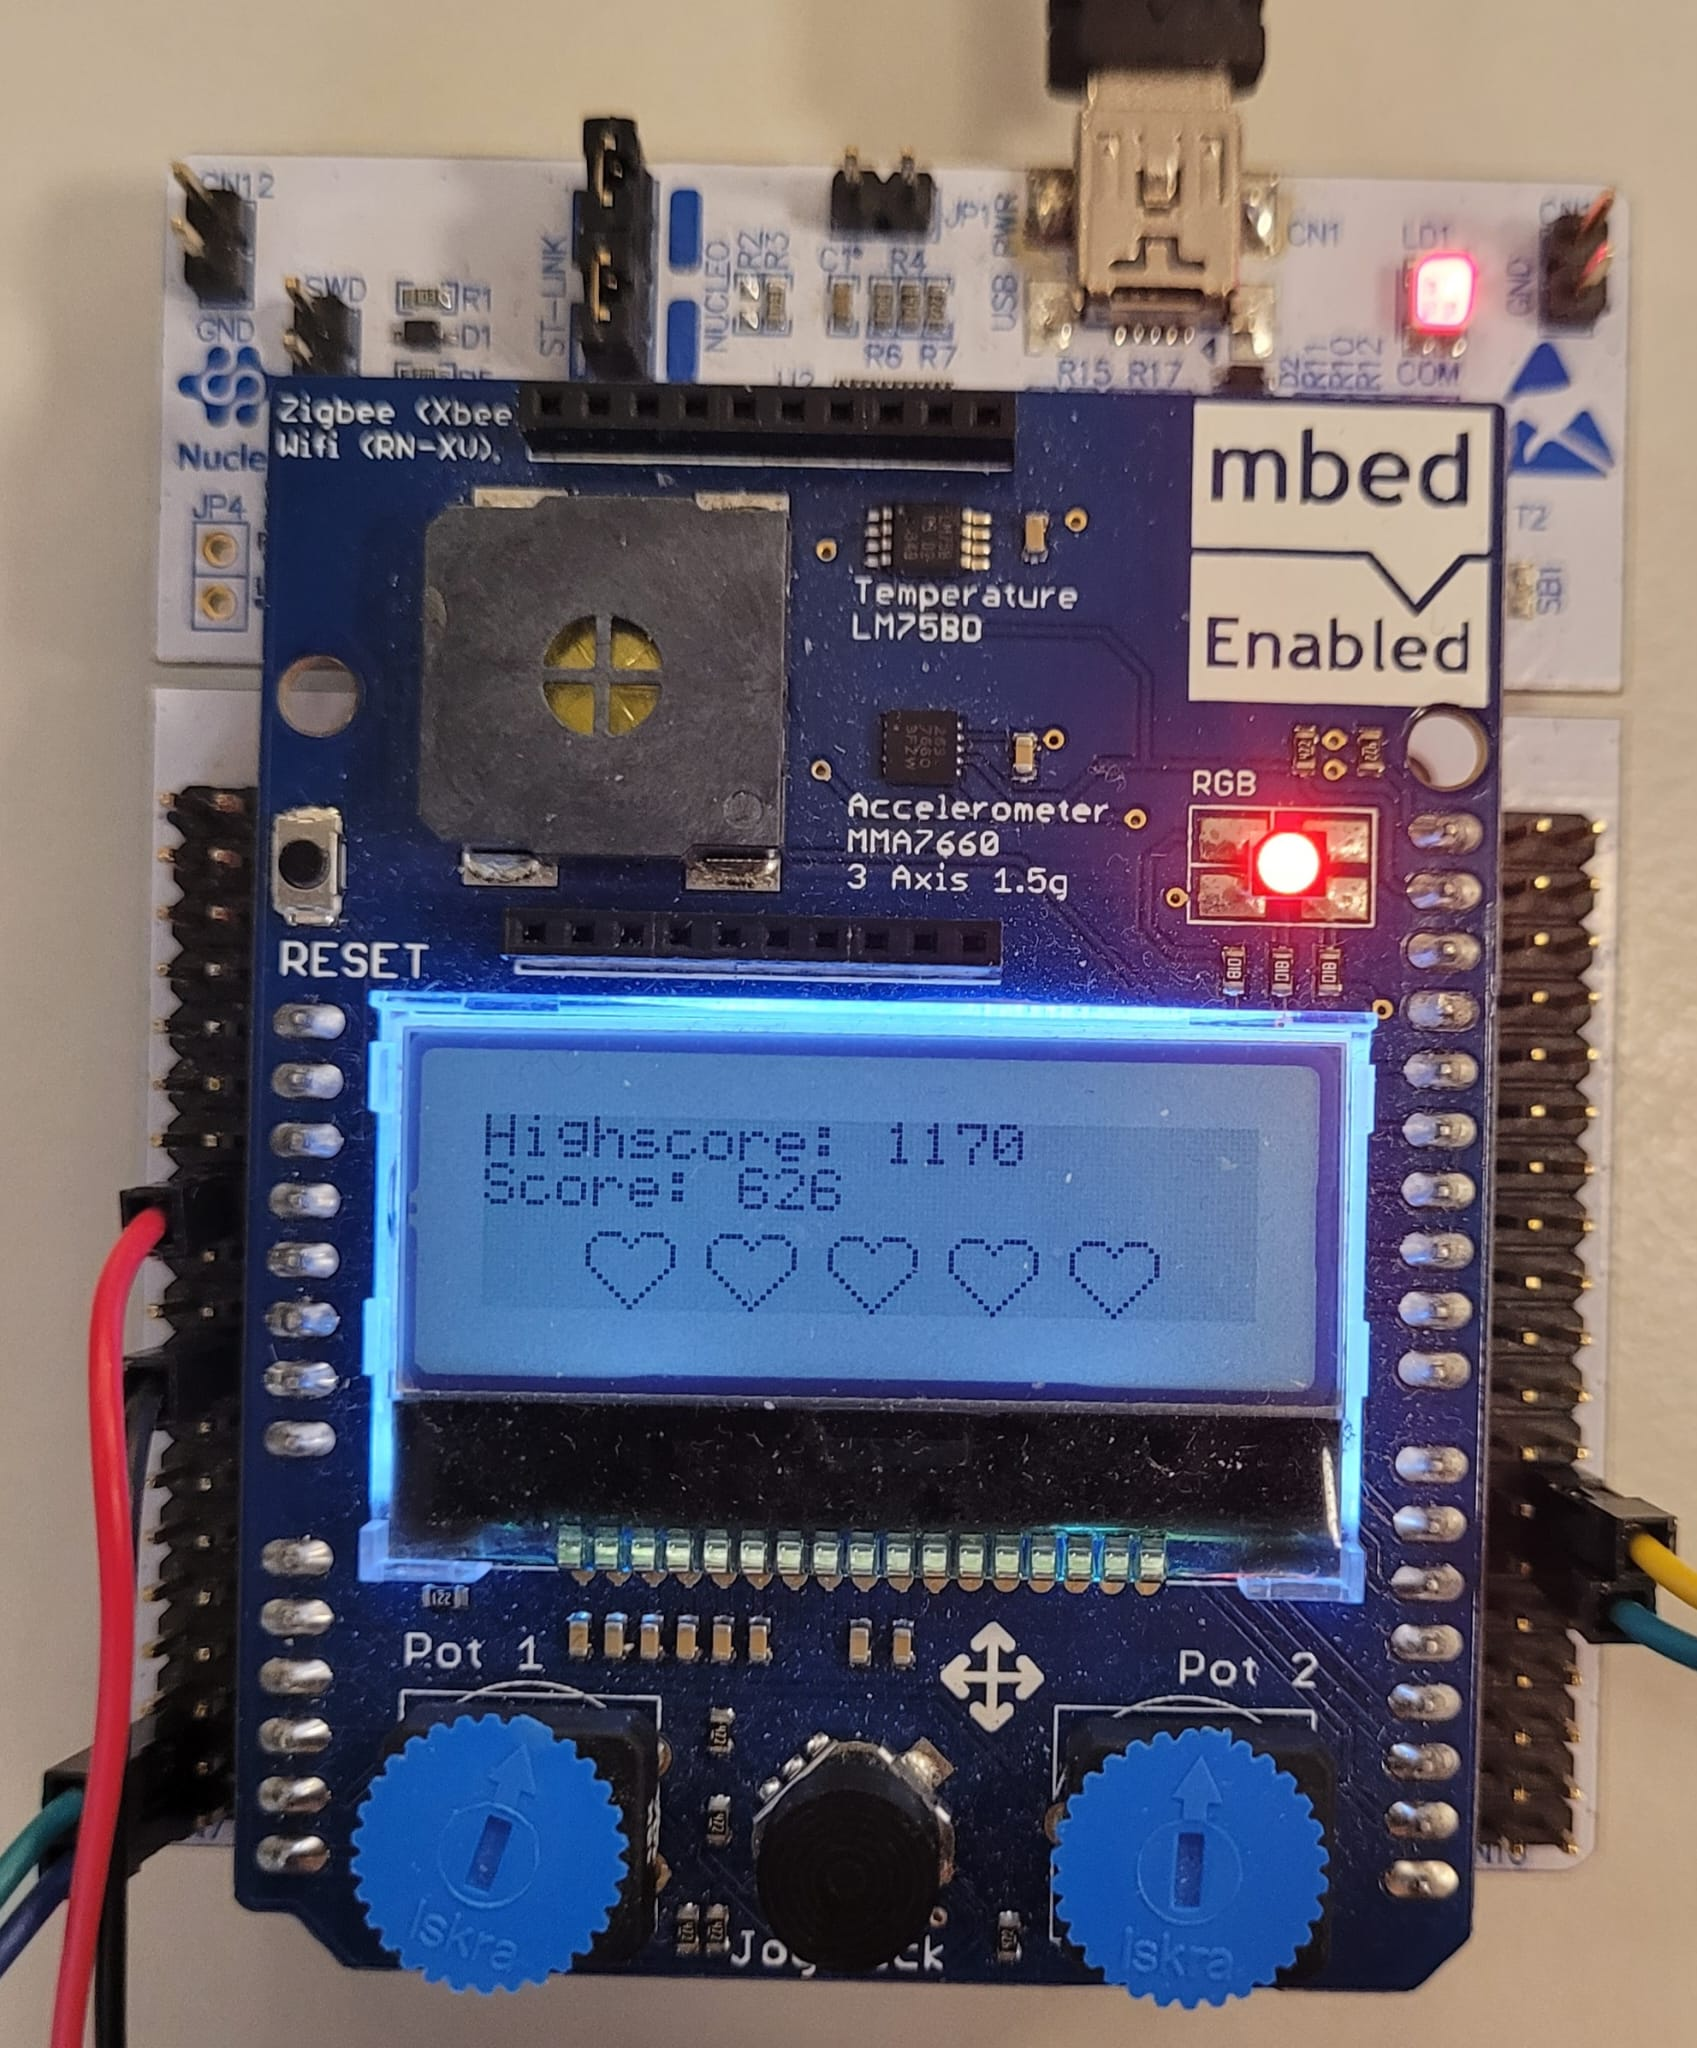
\includegraphics[width=\textwidth]{Picturs/Opsetning/Nucleo.jpeg}
        \caption{Billede af NUCLEO board}
        \label{fig:NUCLEO}
    \end{minipage}
\end{figure}
\vspace{-1em}

For at kunne køre vores program kræver det som sagt en korrekt sammenkobling af hardwaren. Systemet er centreret omkring NUCLEO-F302R8 mikrokontrolleren, hvorpå der er monteret et MBED Extension board. Det eksterne 30010 joystick er essentielt for spillets styring og skal forbindes korrekt til NUCLEO-boardet for at sikre at de analoge og digitale signaler modtages korrekt. Joysticket forbindes til porte på NUCLEO-boardet som følgende angivet (Hardware konfigurationen kan ses på figur \ref{fig:hardware_konfiguration} på næste side): 

\vspace{2em}
\textbf{Strømforsyning:} For aktivere joysticket forbindes VDD på joysticket til 3.3V på NUCLEO boardet, men GND forbindes til Ground.

\vspace{-0.5em}
\textbf{Analog akser (ADC):} ADC1 forbindes til port PC\_3, og ADC2 forbindes til PC\_2. 

\vspace{-0.5em}
\textbf{Digitale knapper:} B1 og B2 forbindes til henholdsvis PA\_6 og PA\_7.

\begin{figure}[H]
    \centering
    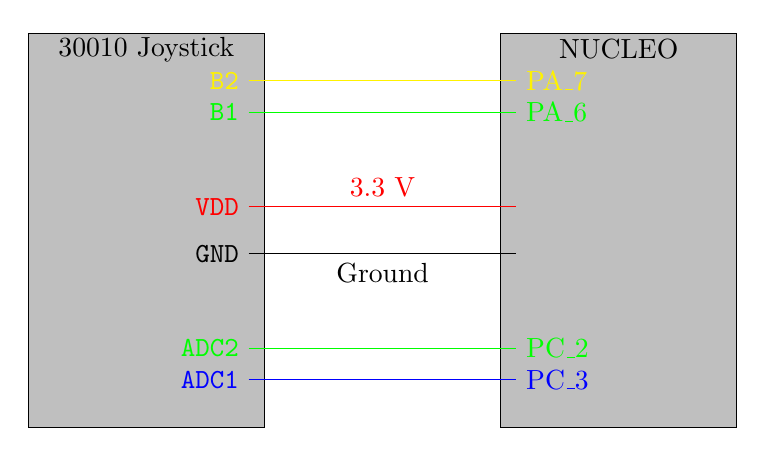
\begin{tikzpicture}
  \draw[fill=lightgray] (0,0) rectangle (3,5);
  \draw[fill=lightgray] (6,0) rectangle (9,5);
  \draw[color=blue] (2.8,0.6) node[left] {\texttt{ADC1}} -- (6.2,0.6) node[right] {PC\_3};
  \draw[color =green] (2.8,1) node[left]{\texttt{ADC2}} -- (6.2,1) node[right] {PC\_2};
  \draw[color=black] (2.8,2.2) node[left] {\texttt{GND}} -- node[below] {Ground} (6.2,2.2);
  \draw[color=red] (2.8,2.8) node[left] {\texttt{VDD}} -- node[above]{3.3 V} (6.2,2.8);
  \draw[color=green] (2.8,4) node[left] {\texttt{B1}} -- (6.2,4) node[right] {PA\_6};
  \draw[color=yellow] (2.8,4.4) node[left] {\texttt{B2}} -- (6.2,4.4) node[right] {PA\_7};
  \node at (7.5,4.8) {NUCLEO};
  \node at (1.5,4.8) {30010 Joystick};
\end{tikzpicture}
    \caption{Hardware konfiguration}
\label{fig:hardware_konfiguration}
\end{figure}
\vspace{-1em}

Joystikets pins kan aflæses på selve 30010 Joysticket, som vis på billede \ref{fig:30010}. De tilsvarende pins på NUCLEO-F302R8 mikrokontrolleren kan aflæses fra STM32F302x8\_NUCLEO\_F302R8\_Pinout pin diagrammet, som kan ses i Appendix \ref{chap:appendiks_1}.

\section{Putty-indstillinger}
\vspace{0.5em}

For at spillet kører smooth og efter hensigten, skal PUTTY terminalen indstilles efter disse bekrivelser.
\begin{itemize}
    \setlength{\itemsep}{4pt}
    \setlength{\parskip}{0pt}
    \setlength{\parsep}{0pt}
    \item Session \rightarrow Serial line: <din serial forbindelse> 
    \item Connnection type: Serial
    \item Speed: 950000
    \item Window \rightarrow set size of window \rightarrow Columns: 100, Rows: 32
    \item Window \rightarrow Translation \rightarrow Remote character set: CP850 
\end{itemize}

\section{Kør Spillet} 
\label{chap:Brugermanual_sec:software}
\vspace{0.5em}

Nu kan spillet køres på mikrocrontrolleren. 
\begin{itemize}
    \setlength{\itemsep}{4pt}
    \setlength{\parskip}{0pt}
    \setlength{\parsep}{0pt}
    \item Download spillet enten via zip på learn eller på \href{https://github.com/wrl6765/DTU-30010-Gruppe-13}{GitHub}
    \item Åben main.c inden i STM32Cube IDE eller din yndlings mikrocontroller konfigurerings app.
    \item sæt configure til AUTO
    \item åben PUTTY med indstillinger fra tidligere sektion og kør koden
\end{itemize}

Sådan! Så brude spillet gerne være sat i gang. Der opfordres til at prøve alle menuer og powerups, samt at forsøge at få en highscore over 1000, så man får den fulde oplevelse.
